No capítulo anterior foram abordadas as soluções EKF e SEIF, com maior 
foco neste último, do problema de estimação que deve ser resolvido por um 
sistema SLAM. Mas apenas resolver a estimação não é suficiente, existem 
outras capacidades ``comportamentais'' que um robô deve possuir para 
performar SLAM, como: processamento de leituras dos sensores, construir 
representações úteis do ambiente e, a partir dessas representações traçar 
trajetórias a fim de explorá-lo e aumentar seu conhecimento a respeito 
do mesmo. Todos esses aspectos são compreendidos pelo \textit{front end} 
como mostrado na Figura \ref{fig:slam-architecture}, e nesse capítulo serão abordadas as soluções para alguns de seus componentes.

\section{Dados do sensor laser}
Essa Seção explica o formato dos dados brutos do sensor LiDAR, e como eles 
são processados e transformados nos dados utilizados pelo modelo de medida 
descrito na Seção \ref{sec:slam-measurement} (\nameref{sec:slam-measurement}).

\subsection{Dados brutos}
Os dados brutos do sensor LiDAR utilizado, consistem numa sequência de 
distâncias $\{r^0, r^1, \dots, r^N\}$. Esses valores são gerados pela reflexão de feixes de laser, emitidos pelo sensor, nas superfícies 
presentes no ambiente. Os feixes são disparados de maneira sequencial no 
sentido anti-horário, a partir do eixo $x$ do sistema de coordenadas do sensor. 
Além disso, o sensor também fornece as posições angulares $\theta_0$ 
do primeiro e $\theta_N$ do último feixe, e o incremento na posição angular $\Delta \theta$ entre o feixe $k$ e o feixe $k+1$.

A Figura \ref{fig:sensor-raw-data} apresenta os dados brutos obtidos em uma 
leitura feita no ambiente mostrado na Figura \ref{fig:environment}.
\begin{figure}[]
  \centering
  \begin{subfigure}{0.39\textwidth}
    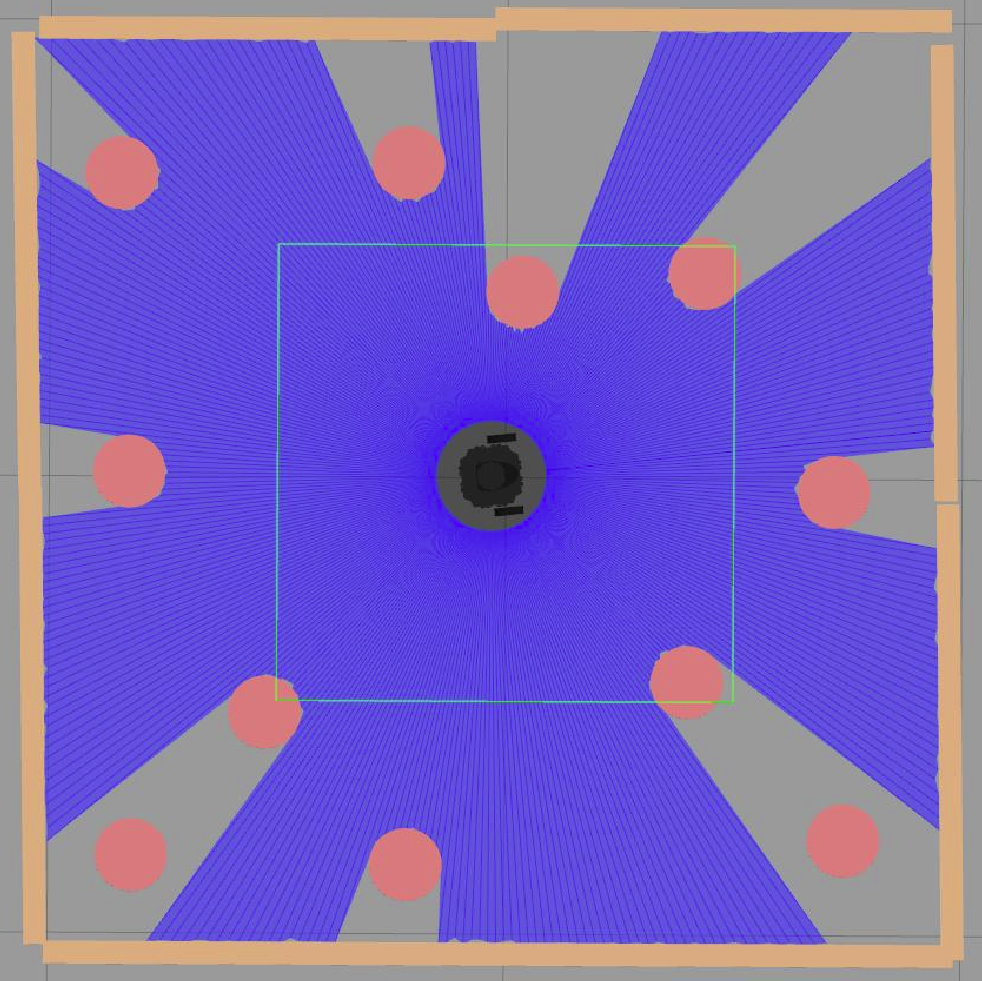
\includegraphics[width=\textwidth]{figs/sensor-simulation-view-tiny.png}
    \caption{Representação dos feixes laser (em azul) emitidos pelo sensor LiDAR com 
    alcance máximo de 2 metros. Os círculos em rosa representam as landmarks.}
    \label{fig:laser-beams-visualization}
  \end{subfigure}
  \hfill
  \begin{subfigure}{0.60\textwidth}
    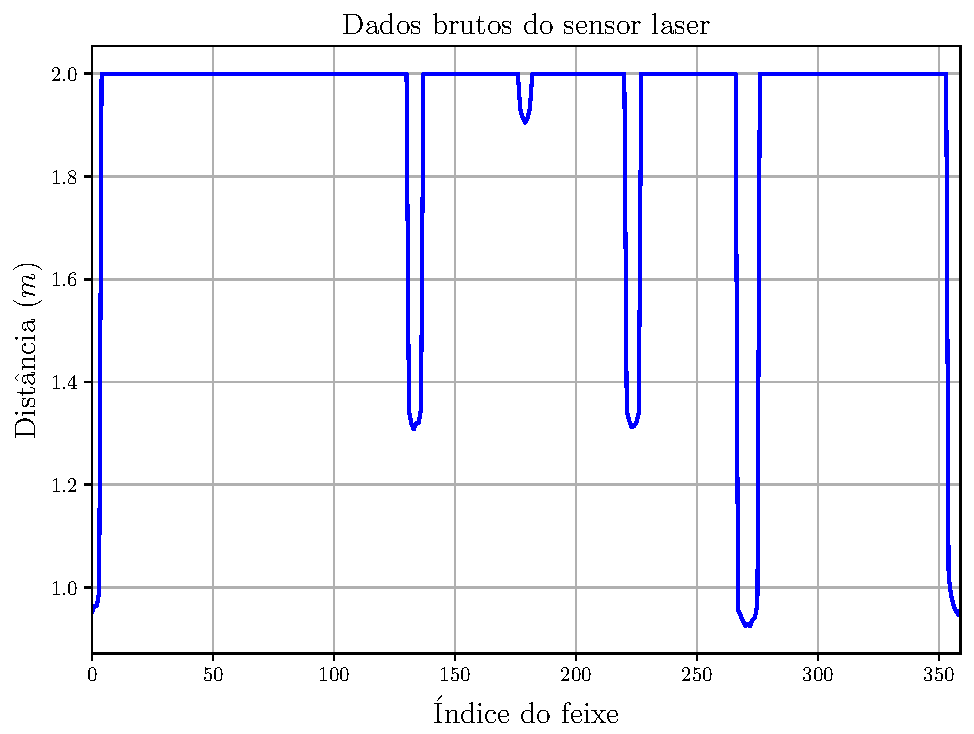
\includegraphics[width=\textwidth]{figs/raw_sensor_data.pdf}
    \caption{Interpolação linear das distâncias lidas pelo sensor.}
    \label{fig:sensor-raw-data}
  \end{subfigure}
  \caption{Visualização dos feixes laser emitidos pelo sensor LiDAR e a 
  respectiva leitura gerada.}
  \label{fig:sensor-visualization-and-reading}
\end{figure}

\subsection{Processamento de dados}
Para transformar o dado bruto, a sequência de distâncias na Figura 
\ref{fig:sensor-raw-data}, nas medidas consumidas pelo modelo de medida 
descrito na Seção \emph{\nameref{sec:slam-measurement}}, é proposto um 
\textit{pipeline} de processamento de dados, Figura \ref{fig:lidar-data-processing-pipeline},cujo último estágio é o 
algoritmo de estimação de círculos a partir de pontos em coordenadas 
cartesianas \cite[p.~903]{al2009error}.

\begin{figure}[]
  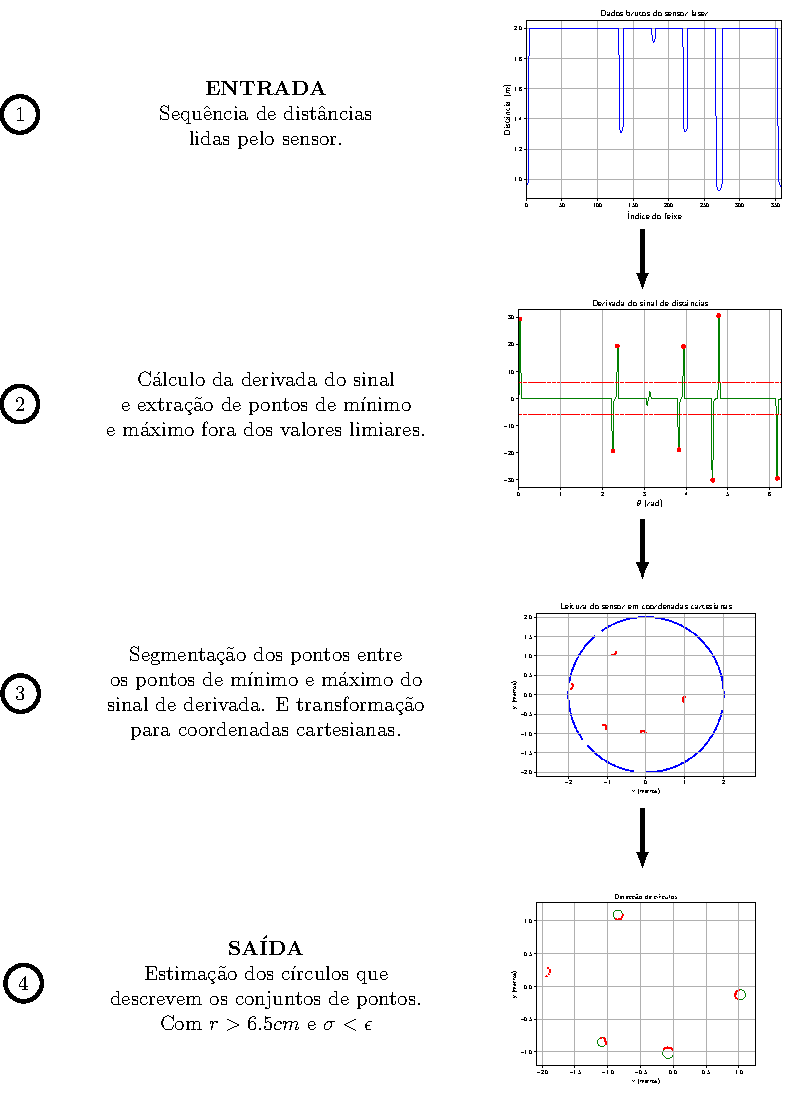
\includegraphics[width=\textwidth]{figs/data_processing_pipeline.pdf}
  \caption{Sequência de passos para processar os dados brutos do sensor LiDAR e
  transforma-los em dados úteis para o modelo de medida utilizado.}
  \label{fig:lidar-data-processing-pipeline}
\end{figure}

Para começar, é necessário extrair os pontos que correspondem às reflexões nas 
superfícies dos cilindros presentes no ambiente. Para isso, observa-se que há uma variação brusca nas distâncias lidas pelo sensor quando os feixes são 
refletidos pelas superfícies dos cilindros. Ao analisar a derivada do sinal, 
representada na Figura \ref{fig:sensor-derivative}, podemos notar que o intervalo de medidas 
correspondente às reflexões dos cilindros se encontram entre uma variação 
negativa seguida rapidamente de uma variação positiva na curva da derivada.
\begin{figure}[]
  \centering
  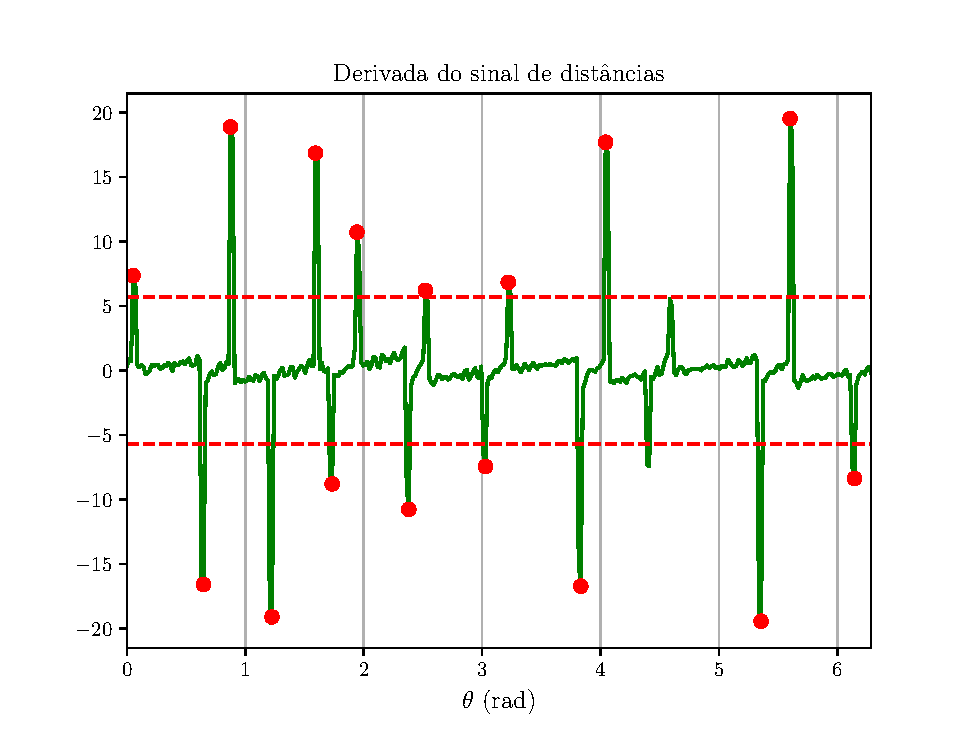
\includegraphics[width=.6\textwidth]{figs/signal_derivative.pdf}
  \caption{Derivada central da sequência de distâncias representadas na Figura \ref{fig:sensor-raw-data}. As linhas pontilhadas em vermelho 
  representam os limiares a partir dos quais os picos são interpretados 
  como início (negativo) ou fim (positivo) da superfície de um cilindro. Os picos destacados 
  em vermelho ultrapassam as valores limiares.}
  \label{fig:sensor-derivative}
\end{figure}

O próximo passo consiste em transformar o sinal para a representação em 
coordenadas cartesianas, e segmentar os conjuntos de pontos correspondentes aos intervalos entre picos e vales do sinal de derivada computado anteriormente, como é mostrado na Figura \ref{fig:sensor-data-cartesian}.
Então, cada um desses conjuntos é fornecido como entrada do Algoritmo 
\ref{alg:circle-fit} (listado no Anexo \ref{annex:circle-fit}), o resultado 
são círculos que melhor explicam esses conjuntos de pontos (Figura \ref{fig:detected-circles}), juntamente com o 
erro médio quadrático entre cada conjunto de pontos e seu círculo.
\begin{figure}[]
  \centering
  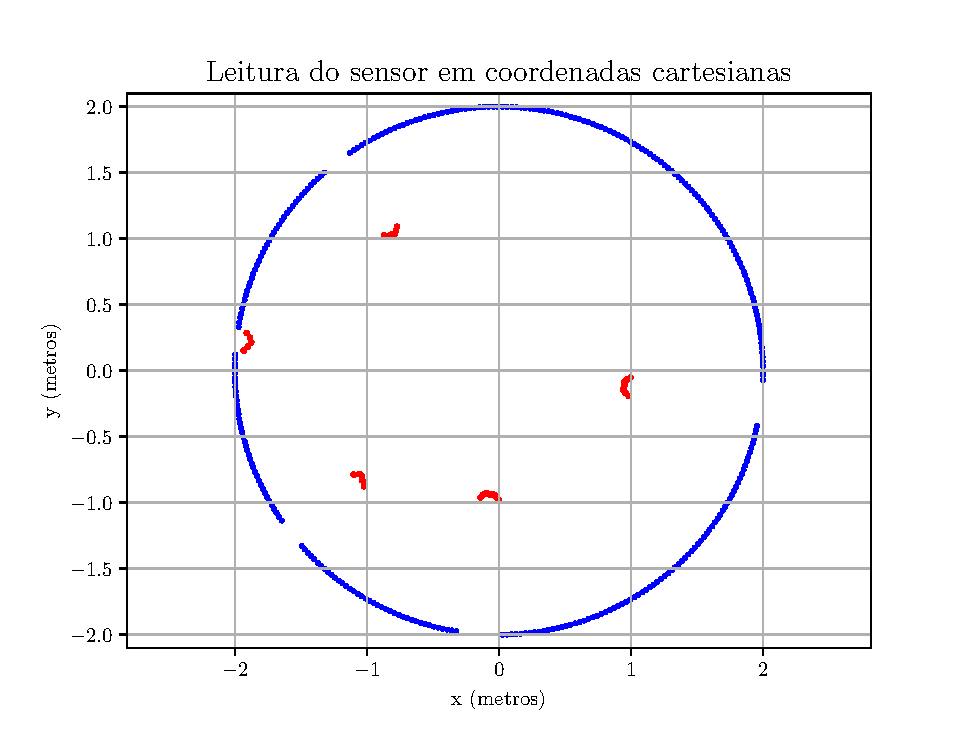
\includegraphics[width=.8\textwidth]{figs/sensor_data_cartesian.pdf}
  \caption{Representação da leitura do sensor LiDAR em coordenadas 
  cartesianas. Os pontos destacados em azul correspondem a reflexões 
  das superfícies das \textit{landmarks}.}
  \label{fig:sensor-data-cartesian}
\end{figure}

Por fim são considerados apenas os círculos cujo erro médio quadrático para 
seus pontos correspondentes é inferior a um limiar $\epsilon = 10^{-3}$ e 
cujo raio seja superior a 6cm. Essa última condição é especialmente útil no 
cenário multiagente, pois evita de que um robô confunda o sensor LiDAR (que 
fica montado no topo do robô, conforme visto na Figura \ref{fig:turtlebot-digital-twin}) do outro com uma \textit{landmark}.

\begin{figure}[]
  \centering
  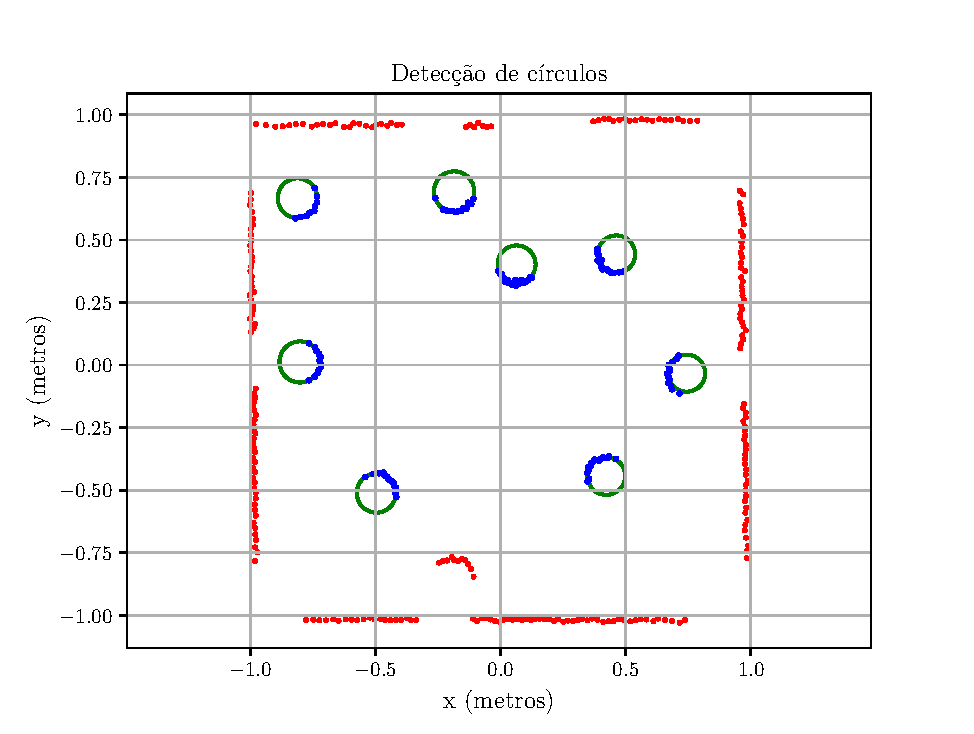
\includegraphics[width=.8\textwidth]{figs/circle_detection.pdf}
  \caption{Em azul, os conjuntos de pontos selecionados como pertencentes à superfícies das \textit{landmarks}. Em verde, os círculos 
  estimados para cada conjunto.}
  \label{fig:detected-circles}
\end{figure}

\section{Mapa em grade}
Até o momento o ambiente foi representado apenas como um conjunto de 
\textit{landmarks}, embora essa representação seja muito útil para a 
estimação, abordada no Capitulo \ref{ch:backend}, ela não é adequada 
para representar outros aspectos do ambiente além das próprias \textit{landmarks}. O robô não consegue representar a presença de outros 
objetos, paredes ou até mesmo outros agentes.

Uma forma de representação que trata desses problemas é a grade de 
ocupação. Grades de ocupação discretizam o espaço em um conjunto de 
células, onde cada célula armazena a probabilidade de estar ocupada ou 
não \cite{elfes1989using}. A Figura \ref{fig:occuopancy-grid-represetation} ilustra a grade de ocupação construída a 
partir das observações a partir do centro da cena representada na Figura 
\ref{fig:laser-beams-visualization}.

Para utilizar grade de ocupação são adotadas duas hipóteses 
simplificadoras: a primeira é que a as células são independentes e o 
estado de ocupação de uma célula não diz nada sobre o estado de outra; a 
segunda é que o ambiente é estático. Embora essas duas premissas sejam 
falsas, grades de ocupação funcionam muito bem na prática inclusive em 
ambientes dinâmicos. A primeira hipótese é falsa porque se uma célula 
representa a ocupação de parte do corpo de um objeto, é muito provável 
que suas vizinhas também estejam ocupadas por esse objeto. E a segunda 
porque porque há outros agentes se movimentando no ambiente.

Utilizando essas hipóteses, cada célula pode ser modelada como uma variável aleatória binária 
que pode assumir os estados livre ou ocupado, e cujo estado é constante 
no tempo (i.e. estático). Isso sugere a utilização 
do filtro de Bayes binário \cite[p.~94]{bongard2006probabilistic} para estimar o estado das células 
da grade.

\begin{figure}[]
  \centering
  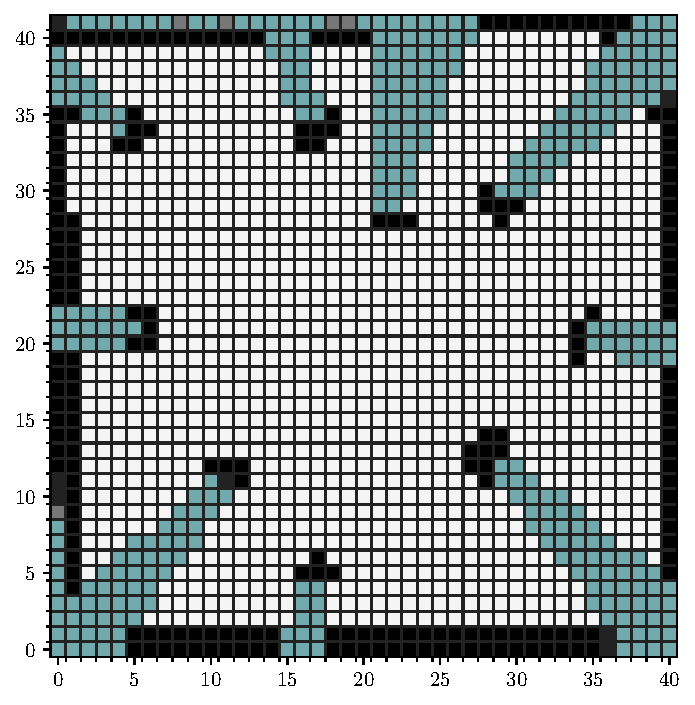
\includegraphics[width=0.6\textwidth]{figs/grid_map_view_vec.pdf}
  \caption{Grade de ocupação produzida utilizando as leituras do sensor LiDAR. As células em azul representam porções do ambiente com estado 
  desconhecido a partir da observação deste único ponto de vista. A 
  cor das demais células refletem a probabilidade de estarem ocupadas,
  quanto mais escura maior a confiança do robô de que existe algum 
  objeto no espaço delimitado pela célula. Cada célula é um quadrado 
  com lado 5cm.}
  \label{fig:occuopancy-grid-represetation}
\end{figure}

\subsection{Construção da grade de ocupação}
Para construir a grade de ocupação primeiro é necessário definir sua 
resolução, isto é, o tamanho de sua célula. Quanto menor a célula, mais 
memória é utilizada para representar o ambiente e melhor é a 
representação. A quantidade de células pode ser fixa, caso a área da 
grade seja definida inicialmente, ou dinâmica.

Uma vez que o ambiente está segmentado em células, utiliza-se o modelo de 
medida inverso \invMeasurementModel (Seção \ref{sec:inverse-measurement-model}) para determinar a qual célula pertence 
a extremidade do feixe da leitura do LiDAR. Caso o comprimento do feixe 
seja menor que o alcance máximo do sensor a probabilidade de ocupação da 
célula, que contém a extremidade do feixe, aumenta. Enquanto as das 
células ao longo do feixe diminui.

Para determinar quais células da grade são interceptadas pelos feixes do 
sensor LiDAR é utilizado o algoritmo de desenho de linha 
de Bresenham \cite{bresenham1965algorithm}. Inicialmente 
esse algoritmo foi criado para desenhar linhas em \textit{plotters} 
digitais, mas ele também pode ser usado para desenhar linhas em grades de 
pixel, como monitores. Aqui ele usado para ``desenhar'' o feixe do 
LiDAR, com origem no sensor e extremidade calculada pelo modelo de medida 
inverso, na grade de ocupação. Então as células utilizadas no desenho são 
as células interceptadas pelo feixe, como é ilustrado na Figura \ref{fig:bresenham-demo}.

\begin{figure}
  \centering
  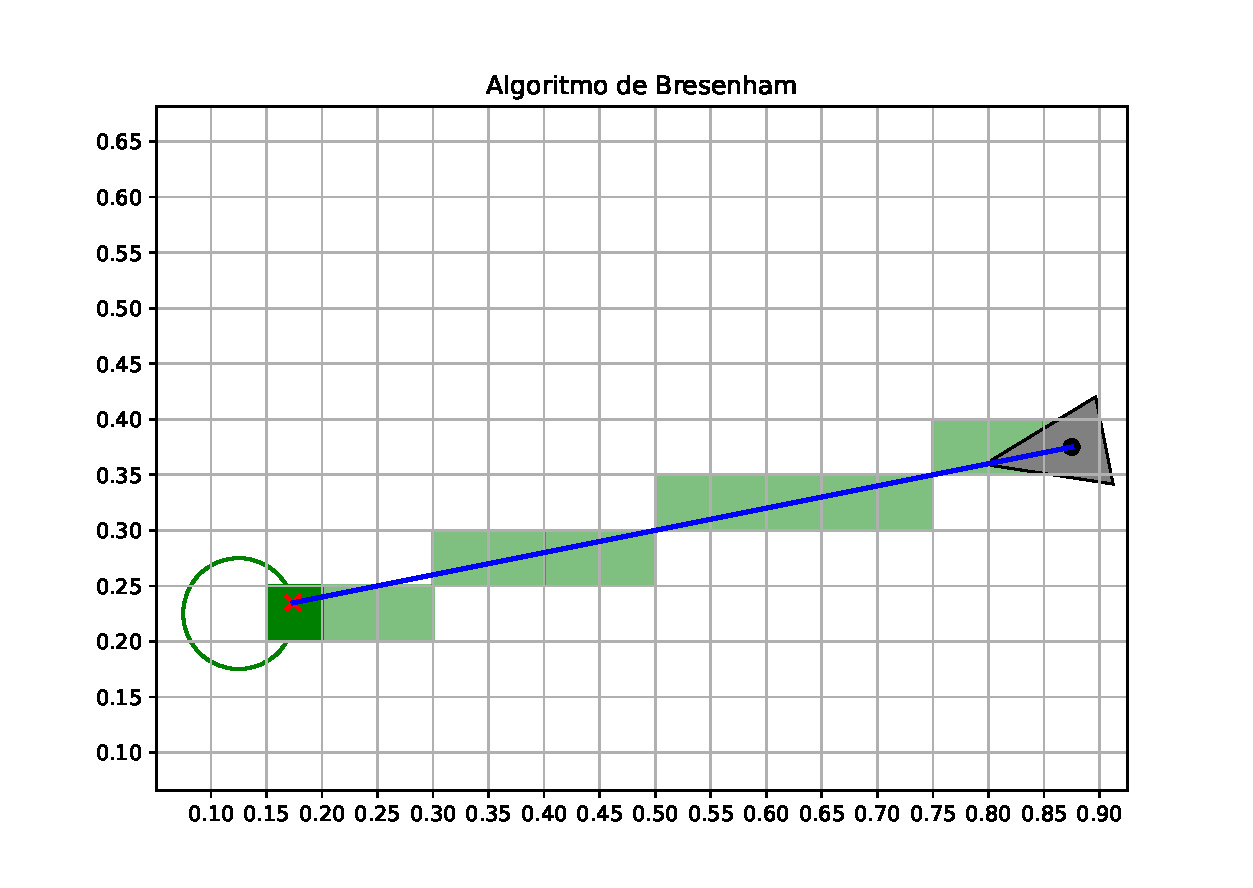
\includegraphics[width=0.8\textwidth]{figs/bresenham_demop.pdf}
  \caption{Uso do algoritmo de Bresenham para determinar as células 
  interceptadas pelo feixe (em azul) do sensor LiDAR. As células em 
  verde claro, representam o espaço atravessado pelo feixe. A célula 
  em verde escuro representam o espaço em que o feixe interceptou a 
  superfície de um objeto. O robô é representado pelo triângulo cinza.}
  \label{fig:bresenham-demo}
\end{figure}

Por fim é preciso definir uma distribuição de probabilidade de ocupação 
das células para o modelo de medida inverso. Por conta da boa precisão 
de sensores do tipo LiDAR utilizou-se um modelo simplificado, ilustrado 
na Figura \ref{fig:simplified-inv-measurement-model}.

\begin{figure}
  \centering
  \includegraphics[width=0.6\textwidth]{figs/inverse-measurement-model-probability.tex}
  \caption{Distribuição de probabilidade simplificada do modelo de 
  medida inverso.}
  \label{fig:simplified-inv-measurement-model}
\end{figure}

\subsection{Representação em \textit{log odds}}
Implementações do filtro de Bayes binário são comumente realizadas na 
forma do logaritmo da razão de chances (\textit{log odds ratio}) \cite[p.~94]{bongard2006probabilistic}. A razão de chances, ou \textit{odds} é a 
razão entre a probabilidade de ocorrência de um evento (a célula 
estar ocupada), dividida pela razão da não ocorrência desse evento (a 
célula estar livre). Se $\pr{c_{ij} \given \bsubvec{y}{1:t}}$ é a probabilidade da célula $c_{ij}$ 
estar ocupada dada as medidas dos sensor LiDAR até o instate $t$, então a sua razão de chances é:
\begin{equation}
  \frac{\pr{c_{ij}\given \bsubvec{y}{1:t}}}{\pr{\neg c_{ij}\given \bsubvec{y}{1:t}}} = \frac{\pr{c_{ij}\given \bsubvec{y}{1:t}}}{1 - \pr{c_{ij}\given \bsubvec{y}{1:t}}}
\end{equation}
A atualização recursiva da razão de chances da ocupação de uma célula é 
dada pelo produto de razões mostrado na Equação \ref{eq:recursive-bayes-filter-update} abaixo \cite[p.~96]{bongard2006probabilistic}. A primeira razão corresponde à razão de 
chances do ocupação do modelo de medida inverso, cuja distribuição de 
probabilidade foi mostrada na Figura \ref{fig:simplified-inv-measurement-model}, o termo do meio é o termo 
recursivo, e o da direita representa algum conhecimento incial que se 
possa ter sobre o ambiente.
\begin{equation}
  \frac{\pr{c_{ij}\given \bsubvec{y}{1:t}}}{\pr{\neg c_{ij}\given \bsubvec{y}{1:t}}} = \frac{\pr{c_{ij}\given \bsubvec{y}{t}}}{1 - \pr{c_{ij}\given \bsubvec{y}{t}}} \frac{\pr{c_{ij}\given \bsubvec{y}{1:t-1}}}{1 - \pr{c_{ij}\given \bsubvec{y}{1:t-1}}} \frac{1 - \pr{c_{ij}}}{\pr{c_{ij}}}
  \label{eq:recursive-bayes-filter-update}
\end{equation}
Definindo o logaritmo da razão de chances, também conhecido por logit, por:
\begin{equation}
  l_{t} = \log\parentheses{\frac{\pr{c_{ij}\given \bsubvec{y}{1:t}}}{\pr{\neg c_{ij}\given \bsubvec{y}{1:t}}}}
\end{equation}
Aplicando a definição acima na 
Equação \ref{eq:recursive-bayes-filter-update}, ela pode ser reescrita 
na forma da Equação \ref{fig:occuopancy-grid-represetation}:
\begin{equation}
  l_t = \log\parentheses{\frac{\text{Modelo-de-medida-inverso}}{1 - \text{Modelo-de-medida-inverso}}} + l_{t-1} - l_0
  \label{eq:occupancy-grid-log-odds}
\end{equation}
E a probabilidade de ocupação de uma célula pode ser recuperada 
utilizando a relação na Equação \ref{eq:log-odds-to-probability}.
\begin{equation}
  p = 1 - \frac{1}{1 + \exp({l_t})}
  \label{eq:log-odds-to-probability}
\end{equation}

Como fica claro na Equação \ref{eq:occupancy-grid-log-odds}, a 
incorporação de novas leituras se resume a uma simples adição. Esse 
aspecto da representação em \textit{log odds} será muito útil mais 
adiante quando os agentes trocarem suas grades de ocupação, pois após 
o alinhamento entre as grades a fusão entre elas também será uma simples 
soma.

\section{Exploração Autônoma}

Na Seção anterior foi mostrado como as grades de ocupação são utilizadas 
para representar ambiente e como essa representação é construída e 
mantida. Nessa seção será mostrado como a grande pode ser empregada para 
determinar regiões alvo para exploração dos agentes e como elas são 
úteis para evitar obstáculos e evitar que os robôs colidam com outros 
objetos.
